\chapter{Perfiles de estudiantes según su rendimiento}
\addcontentsline{toc}{chapter}{Perfiles de estudiantes según su rendimiento}

Debido a la dificultad de predecir de manera exacta la calificación obtenida por los alumnos a partir de las medidas de rendimiento descritas anteriormente, se agruparán las notas en clusters significativos y trataremos de predecir en qué cluster se encuentra la nota de un determinado grupo de alumnos.

\subsection{Por clusters fijos de notas}

En primer lugar, escogeremos como separación los cuartiles de las calificaciones. Así pues, podemos ver la distribución de los cuartiles en la Figura \ref{fig:boxplotgradequartilegrade}, donde los límites inferiores de cada una de las cajas son $6.99$, $8.23$, $8.95$ y $9.60$ respectivamente.

\begin{figure}[H]
    \centering
    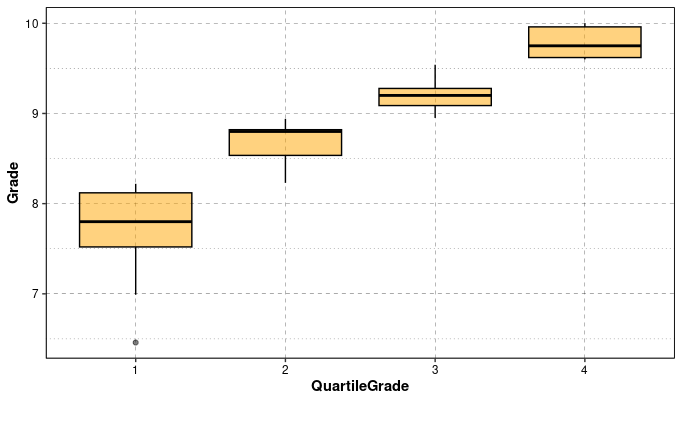
\includegraphics[width=0.6\textwidth]{boxplotgrade.png}
    \caption{Boxplot de las calificaciones por cuartil.}
    \label{fig:boxplotgradequartilegrade}
\end{figure}

Sin embargo, en la Figura \ref{fig:boxplotgradequartilegrade} y en la Figura \ref{fig:frequenciesgrade}, donde se representan cómo de frecuentes son cada una de las calificaciones obtenidas, notamos la presencia de un outlier.

\begin{figure}[H]
    \centering
    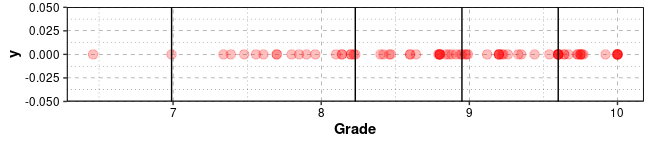
\includegraphics[width=0.6\textwidth]{frequencygrade.png}
    \caption{Calificaciones obtenidas por los distintos grupos. El límite de los cuartiles se ha indicado con líneas verticales negras.}
    \label{fig:frequenciesgrade}
\end{figure}

En la Figura \ref{fig:densitybyfactorquartilegrade} vemos las funciones de densidad por cuartil. Prestaremos especial atención a los grupos del cluster \texttt{Q1} (el de las peores calificaciones al que le añadimos el outlier) puesto que son los que peor rendimiento han mostrado.

\begin{figure}[H]
    \centering
    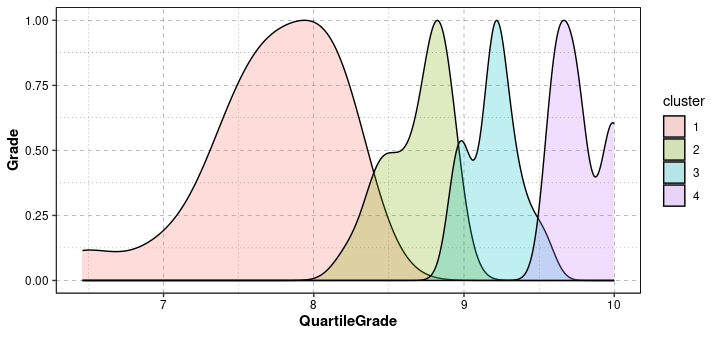
\includegraphics[width=0.6\textwidth]{densitybyfactorquartilegrade.png}
    \caption{Funciones de densidad de las calificaciones obtenidas por cluster.}
    \label{fig:densitybyfactorquartilegrade}
\end{figure}
